\documentclass[]{elsart}
\usepackage[dvips]{graphicx}
\DeclareGraphicsExtensions{ps,eps}
%\graphicspath{{ti1/}{ti2/}{pic/}}

%%%%%%%%%%%%%%%%%%%%%%%%%%%%%%%%%%%%%%%%%%%%%%%%%%%%%%%%%%%%%%%%%%%%%%%%
\begin{document}
\begin{frontmatter}
\title{Variable quality image compression system based on SPIHT}
\author[tucs,tko]{A. J\"{a}rvi\thanksref{corresponding}}
\author[tucs,tko]{J. Lehtinen\thanksref{akatemia}}
\author[tko]{O. Nevalainen}
\address[tucs]{Turku Centre for Computer Science,
Lemmink\"{a}isenkatu 14 A, FIN-20520 Turku, Finland}
\address[tko]{Department of Computer Science,
University of Turku, Lemmink\"{a}isenkatu 14 A, FIN-20520 Turku,
Finland}
\thanks[corresponding]{Corresponding author. E-mail ajarvi@cs.utu.fi,
voice +358 2 3338795, fax +3582 2410154}
\thanks[akatemia]{Joonas Lehtinen acknowledges support by the Academy
of Finland.}

\end{frontmatter}

\newpage
Number of pages is 30.


Number of figures is 10.


Number of tables is 1.


\bigskip
\bigskip
Keywords: Image compression, SPIHT, Wavelet transform, Region of
interest, variable quality image compression, VQIC.

\newpage


%%%%%%%%%%%%%%%%%%%%%%%%%%%%%%%%%%%%%%%%%%%%%%%%%%%%%%%%%%%%%%%%%%%%%%%%
%%%%%%%%%%%%%%%%%%%%%%%%%%%%%%%%%%%%%%%%%%%%%%%%%%%%%%%%%%%%%%%%%%%%%%%%
{\bf Abstract}

\bigskip
             
   
\noindent An algorithm for variable quality image compression is
given. The idea is to encode different parts of an image with
different bit rates depending on their importance. Variable quality
image compression (VQIC) can be applied when {\em a priori} knowledge on some
regions or details being more important than others is available. Our
target application is digital mammography, where high compression
rates achieved with lossy compression are necessary due to the vast
image sizes, while relatively 
small regions containing signs of cancer must remain 
practically unchanged. We show how VQIC can be
implemented on top of SPIHT~\cite{SPIHT}, an embedded wavelet encoding 
scheme. We have revised the algorithm to use matrixes, which gives
more efficient implementation both in terms of memory usage and
execution time. The effect of the VQIC on the quality of compressed images is
demonstrated with two test pictures: a drawing and a more relevant
mammogram image.

%%%%%%%%%%%%%%%%%%%%%%%%%%%%%%%%%%%%%%%%%%%%%%%%%%%%%%%%%%%%%%%%%%%%%%%%
%%%%%%%%%%%%%%%%%%%%%%%%%%%%%%%%%%%%%%%%%%%%%%%%%%%%%%%%%%%%%%%%%%%%%%%%

 
\section{Introduction}   
                         
%%%%%%%%%%%%%%%%%%%%%%%%%%%%%%%%%%%%%%%%%%%%%%%%%%%%%%%%%%%%%%%%%%%%%%%%
%%%%%%%%%%%%%%%%%%%%%%%%%%%%%%%%%%%%%%%%%%%%%%%%%%%%%%%%%%%%%%%%%%%%%%%%

The number of large digital image archives is increasing rapidly in
many fields, including health care. The cost efficient archiving
causes a need for  high quality image compression techniques aiming
at major savings in storage space and network bandwidth when
transmitting the images. Despite the potentionally critical nature of
medical images, some degeneration of the
image quality must be allowed, since the best \emph{lossless compression}
methods can only about half the size of a typical medical image. For
example a digital mammogram with pixel size of $50 \mu$m is approximately of
size 5000x5000 pixels 
with 12 bits per pixel, and thus needs about 50 Mb for storage without
compression. This clearly demonstrates the need for \emph{lossy compression}.

Lossy image compression methods are usually
designed to preserve perceived image quality by removing subtle
details, that are difficult to see with human eye. The frequent
quality measure  used for evaluation of the distortion in a compressed
image is the \emph{mean square error} (MSE). However, in medical
imaging, the distortion of an image is defined
as the impact that compression causes to diagnostic accuracy, and
finally to clinical actions taken on the basis of the
image~\cite{mammoquality}.  In this application area, there is an
evident conflict between the two opposite goals; achieving high
compression ratio and maintaining diagnostically lossless
reconstruction accuracy. One possible way to alleviate this conflict
is to \emph{design an image compression method that uses lossy
compression, but saves more details in important regions of the image
than in other regions.} General-purpose image
compression methods can also be considered to fit into this scheme;
important regions and details are those, that the human visual system is
sensitive to. In medical imaging, the definition of important regions
involves application specific medical knowledge. Obviously the
accuracy of this knowledge is crucial for good performance of the
system. If the criteria for important regions are too loose, the gain in
compression ratio is lost. On the other hand, with too strict
criteria the quality requirements are not met, since some
important regions are treated erroneously as unimportant. 

Today, the standard in lossy image compression is the
JPEG~\cite{compr-stand} algorithm, which is based on the 
scalar quantization of the coefficients of the windowed Discrete
Cosine Transforms (DCT), followed by entropy coding of the quantization
results. JPEG is generally accepted and works well in most cases, but
because it uses DCT and divides the image into blocks of fixed size,
it may distort or even eliminate small and subtle details. This can be
a serious drawback in digital mammography,
where images contain a large number of diagnostically important small low
contrast details, that must preserve their shape and intensity.

\emph{Wavelet} based image compression methods are popular and some of them
can be considered to be ``state of the art'' in general-purpose lossy image
compression (see~\cite{waveletcompr} for an introduction to the
topic). Wavelet compression methods can be divided into three 
stages: \emph{wavelet transform}, \emph{lossy quantization} and
\emph{encoding} of the wavelet coefficients and \emph{lossless entropy
coding}~\cite{vettereli}. The 
wavelet transform is used to de-correlate the coefficients
representing the image. The transform collects the image energy to
relatively small number of coefficients, compared to the original
highly correlated pixel representation. In the quantization phase this
sparse representation and dependencies between coefficients are exploited with
specially tailored quantization and coding schemes. The widely know
\emph{embedded zerotree encoding} (EZW) by Shapiro~\cite{zerotree} is an excellent
example of such coding scheme, and also a good reference to wavelet based
image compression in general. 

One of the most advanced wavelet based image compression techniques is
SPIHT (Set Partitioning In Hierarchical Trees) by Said and
Pearlman~\cite{SPIHT}. SPIHT is clearly a descendant of EZW using
similar zerotree structure and \emph{bitplane coding}. 
In bitplane coding bits of wavelet coefficients are
transmitted in the order of their importance, 
i.e. the coefficients are encoded gradually with increasing
accuracy. Because of this, the encoding  can be stopped at
any stage. The decoder then approximates the values of the original
coefficients with precision depending on the number of bits coded for
each coefficient. This
property called \emph{embedded coding} is the main reason for choosing
SPIHT as the basis of the \emph{Variable Quality Image
Compression system} (VQIC). The implementation of variable quality property is
straightforward in embedded coding: the encoding of the coefficients of the
whole image is ceased somewhere in the middle, and subsequently only bits
of coefficients that influence the important regions are
encoded. 

Another reason for choosing SPIHT is that it appears to
perform very well in terms of compression ratio; in the case of
digital chest X-rays, a compression ratio of 40:1 has been reported to
cause no significant difference when compared to the original in a
radiologist evaluation~\cite{medSPIHTeval}. In an other study SPIHT
compression of mammograms to ratio 80:1 has been found to yield image
quality with no statistically significant differences from the
original mammogram~\cite{perlmutter}. A further indication of good
performance is the fact that the output of SPIHT encoding is so dense,
that additional compression with lossless entropy coding gives an
extra gain of only few percentages \cite{SPIHT}. 

VQIC technique can be applied to any image that is spatially
segmentable to a set of regions that must be saved in better
quality. We do not cover the segmentation problem in this paper
since it is completely application specific. Since we are targeting
at applications where important regions are small, the segmentation is 
done with some kind of feature detector. The feature detection task
for VQIC purpose is considerable easier compared to
applications, where the interest is in the presence or absence of the
feature. In VQIC, a moderate number of false positive detections can be 
tolerated, as long as all of the true features are detected. Thus most
existing feature detection algorithms are suitable, because they can be tuned
to be oversensitive. Several suitable fully automatic segmentation methods
exists for this purpose in the field of medical imaging \cite{giger}, especially for
mammography \cite{detection}. 

Before describing further details, we briefly discuss relevant
research. VQIC has been used in the compression of image sequences in video
conferencing \cite{plompen}. In this work, the pixel values are predicted and the
prediction errors are transformed by 2D-DCT. Coefficients of the blocks 
with minor importance are quantized with coarser level than more
important details, heads and shoulders. In another research, the
importance of a region is 
determined on the basis of the visibility of distortions to human
eye~\cite{meer}. This information is used in the construction of a constant 
quality MPEG stream by adjusting quantization parameters defined by
the MPEG standard. The focus in both papers is the segmentation of
important regions, and VQIC is achieved by variable quantification of
DCT coefficients. A 
recent paper by D. Shin, H. Wu and J. Liu describes a selective
compression technique, which   
integrates detection and compression algorithms into one
system~\cite{shin}. The compression technique used is intraband coding
of wavelet packet transform coefficients, where variable quality is
achieved by scaling the wavelet coefficients in important regions to
increase their priority in coding. The method is tested with a digital
mammogram, where detected microcalcifications are considered as
ROIs. Even though the aims of this work are close to ours,
the actual methods differ considerably.

Our work is organized as follows. In section two we introduce an
algorithm called \emph{variable quality SPIHT}
(\emph{vqSPIHT}), which is basically a reimplementation of SPIHT, with the
added VQIC functionality. We revise the memory
organization of SPIHT to use matrix-based data structures. This new
implementation reduces the working storage requirements of the
algorithm considerably. In section three we discuss the compression
performance of vqSPIHT algorithm, and show with two examples that it
can be superior to SPIHT or JPEG. We first demonstrate
this with a set of details in a high contrast drawing
compressed to  several bit rates with  all three compression
algorithms. We also discuss a more relevant application for VQIC --
 compression of digital mammograms, and make a  comparison between
SPIHT and vqSPIHT compressed images.



%%%%%%%%%%%%%%%%%%%%%%%%%%%%%%%%%%%%%%%%%%%%%%%%%%%%%%%%%%%%%%%%%%%%%%%%
%%%%%%%%%%%%%%%%%%%%%%%%%%%%%%%%%%%%%%%%%%%%%%%%%%%%%%%%%%%%%%%%%%%%%%%%

\section{vqSPIHT algorithm}

%%%%%%%%%%%%%%%%%%%%%%%%%%%%%%%%%%%%%%%%%%%%%%%%%%%%%%%%%%%%%%%%%%%%%%%%
%%%%%%%%%%%%%%%%%%%%%%%%%%%%%%%%%%%%%%%%%%%%%%%%%%%%%%%%%%%%%%%%%%%%%%%%

In this section we explain informally the basic ideas behind
SPIHT and vqSPIHT algorithms to facilitate the reading of the vqSPIHT
algorithm in a pseudo-code format. We also discuss the implementation
based on matrix data structures and its implications to practical
memory requirements. 


%%%%%%%%%%%%%%%%%%%%%%%%%%%%%%%%%%%%%%%%%%%%%%%%%%%%%%%%%%%%%%%%%%%%%%%%
\subsection{Structure of the wavelet transformed coefficient table}
%%%%%%%%%%%%%%%%%%%%%%%%%%%%%%%%%%%%%%%%%%%%%%%%%%%%%%%%%%%%%%%%%%%%%%%%

Wavelet transform converts an image into a coefficient table with
approximately the same dimensions as the original image. 
Fig.~\ref{pyramids} shows the
structure of the \emph{wavelet coefficient table}, which contains three
wavelet coefficient pyramids (pyramids $A$, $B$ and $C$)
and one table of \emph{scaling coefficients} $S$. The scaling
coefficients represent roughly the mean values of larger parts of the
image and wavelet coefficient details of various sizes. Since in
practice the transform is stopped before scaling table $S$ would shrink
to a single coefficient, table $S$ looks like a miniature version of the
original image. The top levels of the three wavelet pyramids are
located adjacent to the scaling table (level three in
Fig.~\ref{pyramids}), and contain coefficients representing large
details, whereas coefficients at level zero contribute mainly to
the smallest details in the image. Pyramid $A$ contains coefficients for
vertical details and pyramid $B$ respectively for horizontal
details. The third pyramid $C$  contains correction coefficients needed
in the reconstruction of the image from pyramids $A$, $B$ and table $S$. 

In the SPIHT algorithm, the pyramids are divided into
\emph{sub-pyramids} which corresponds to zerotrees in EZW. A
sub-pyramid has a top element somewhere in the coefficient table, and
contains four coefficients one level lower in the
corresponding spatial location in the same pyramid, 16 elements two
levels lower, and so on. The sub-pyramids are extended to the scaling
coefficients $S$ in the following way. The scaling coefficients are
grouped into groups of four. The coefficient in the upper left corner
has no descendants, whereas the three remaining coefficients in the
group (upper right corner, lower left corner and lower right corner)
serve as top elements of three sub-pyramids in pyramids $A$, $B$ and
$C$ in corresponding order.

In our approach to VQIC we must determine which coefficients
contribute to the value of a given pixel in the original image. 
In an \emph{octave-band decomposition}, which we use, a coefficient of
any pyramid in higher level corresponds to four coefficients in the
next level at same spatial location.  We use this rule of multiples of
four in choosing important coefficients. 

%%%%%%%%%%%%%%%%%%%%%%%%%%%%%%%%%%%%%%%%%%%%%%%%%%%%%%%%%%%%%%%%%%%%%%%%
\subsection{The basic functioning of SPIHT}
%%%%%%%%%%%%%%%%%%%%%%%%%%%%%%%%%%%%%%%%%%%%%%%%%%%%%%%%%%%%%%%%%%%%%%%%

To understand how SPIHT works, one must keep in mind that it is not a
complete image compression scheme, but a method tailored for optimal
embedded encoding of wavelet transformed image coefficients. The
encoding is optimal in the sense of MSE. SPIHT does not presuppose any
particular wavelet transform.  The only requirement is that the
transform has the octave band decomposition structure, as described
above. Also, the optimal encoding with respect to MSE is achieved
only if the transform is unitary, which is the case in \emph{orthogonal and
biorthogonal} wavelet transforms~\cite{vettereli}. In the implementation
of vqSPIHT, we use biorthogonal B97 wavelets \cite{vettereli}.

\subsubsection{Bitplane coding in SPIHT}

Optimal progressive coding of SPIHT is implemented with a \emph{bitplane
coding scheme}. The order of coding is based on the energy saving
property of unitary transforms, here the wavelet transform. This
property states that the larger the wavelet coefficient is, the more
its transmission reduces the MSE. Furthermore, since SPIHT uses
uniform scalar quantization, transmission of a more significant bit in
any coefficient reduces the MSE more than transmission of a less
significant bit in a possibly larger coefficient~\cite{SPIHT}. 

According to this principle, all coefficients are sorted to a
decreasing order by the \emph{number of significant bits}. The number of
significant bits in the coefficient having the largest absolute value
is noted by $n$. The output is generated by transmitting first all the
$n$:th bits in coefficients that have at least $n$ significant bits,
then $(n-1)$:th bits of coefficients that have at least $(n-1)$
significant bits, and so on. Because the most significant bit of a
coefficient is always one, the sign of the coefficient is transmitted
in place of the most significant bit.

In addition to transmitted bitplanes, 
 the sorting order and the length of each bitplane are needed in the
decoder to 
resolve the location of each transmitted bit in the reconstructed
wavelet coefficient table. This information is not transmitted
explicitly, instead the same algorithm is used in both the encoder and
the decoder, and all branching decisions made in the encoder are
transmitted to the decoder. The
branching decisions are transmitted interleaved with the bitplane
coded bits 
and the signs of coefficients. Because of progressive nature of SPIHT
coding, the transmitted 
bit stream can be truncated at any point and the original coefficient
matrix  approximated with optimal accuracy with respect to the number
of transmitted bits. For each coefficient, the most significant not
transmitted bit is set to one, and the rest to zero, thus achieving a
good approximation in uniform quantization.

\subsubsection{Exploitation of the pyramid structure of wavelet transform}

An important property in most natural images is that the low- and high
frequency components are spatially clustered together. This means in
the wavelet coefficient pyramid, that there is high correlation
between the magnitudes of the coefficients of different levels in
corresponding locations. Also, since the 
variance of the frequency components tends to decrease with increasing
frequency, it is very probable that the coefficients representing fine
details in a particular spatial location will be small, if there is a region
of small coefficients in the corresponding location on coarser level
of the pyramid. Thus it is probable that there exists sub-pyramids
containing only zeroes on the current bitplane. These
\emph{zerotrees} can be encoded with one bit, thus cutting down the number
of sorting decisions considerably and also the branching
decisions that must be transmitted to the decoder. The way these
dependencies between coefficients are exploited in
SPIHT coding is described in the presentation of vqSPIHT
algorithm.


%%%%%%%%%%%%%%%%%%%%%%%%%%%%%%%%%%%%%%%%%%%%%%%%%%%%%%%%%%%%%%%%%%%%%%%%
\subsection{The vqSPIHT algorithm}
%%%%%%%%%%%%%%%%%%%%%%%%%%%%%%%%%%%%%%%%%%%%%%%%%%%%%%%%%%%%%%%%%%%%%%%%


\subsubsection{Extension of SPIHT to vqSPIHT}

To expand the SPIHT algorithm to vqSPIHT, we define a \emph{Region Of
Interest} (ROI) as a region in the image that should be preserved in better
quality  than the rest of the image. 
ROIs can be presented as a binary map that is highly compressible with 
simple run-length encoding and thus does not affect bit rate significantly.

In selective coding mode of vqSPIHT, only coefficients affecting ROIs
are coded. This mode is
triggered when a certain \emph{percentage} $\alpha$ \emph{of the wanted final
output file size} has been reached.  
The choice of $\alpha$ is important, and its best value is highly
application dependent. Some applications might demand more
sophisticated definition of $\alpha$ depending on the file size, area
of the ROIs and some indicator on how ROIs are scattered, for
example. 

To implement selective coding, we construct a
\emph{look-up-table} (LUT), that is used in the function
$influence(i,j)$ defining whether a coefficient $(i,j)$
contributes to any ROI or not. The LUT is constructed by scaling each level of
all three pyramids to the same size as the original image, and
comparing the map of ROIs to the scaled levels. All the coefficients
that overlap with any ROI are marked in the LUT.


\subsubsection{Implementation with matrices}

Instead of lists that are used in the original implementation of
SPIHT, our implementation of vqSPIHT uses two matrices for keeping
track of significant and insignificant coefficients and
sub-pyramids. With the matrix data structures we can considerably
reduce  the working storage requirements of encoding  and decoding.


We introduce a \emph{Point Significance Matrix} (PSM) to indicate
whether a coefficient is known to be $significant$,  $insignificant$
or still  has an $unknown$ state. The labels of PSM are coded
with two bits and the dimensions of the PSM are the same
as in the coefficient table. We also need a \emph{Sub-Pyramid List Matrix}
(SPLM), which is used for maintaining an implicit list of the
sub-pyramids containing only insignificant coefficients. The list
structure is needed, because the order of sub-pyramids must be
preserved in the sorting algorithm. The dimensions of the SPLM are
half of the dimensions of the coefficients matrix, because the
coefficients on the lowest
level of the pyramids can not be top elements of sub-pyramids. 
There are two types of
sub-pyramids. A sub-pyramid of type \emph{A} contains all descendants of
a particular coefficient, excluding the top coefficient
itself. A sub-pyramid of type \emph{B} is otherwise similar, but the 
immediate offspring of the top coefficient is  excluded in addition to
the top coefficient. The list structure with SPLM is simple: the 
lower bits of an element tells the index of the next element in the list.
The type of the sub-pyramid is coded with the highest bit.


\subsubsection{Pseudo-code of vqSPIHT}


The algorithms for the encoder and the decoder are similar. We
use notation ``input/output $x$'', which consists of two steps:
In the encoder $x$ is first calculated and then transmitted to entropy
coder; in the decoder $x$ received from decoder and then used in the
construction of a new estimate for the coefficient. 
Variable $nbc$ indicates the  number of bits transmitted or received thus far. 
Constant $filesize$ indicates the requested final file size in bits.

Function $influence(i,j)$ is defined to be \emph{true}, if the element
$(i,j)$ in the LUT is marked to influence an ROI, and \emph{false}
otherwise. Let
$c_{i,j}$ be the value of the coefficient $(i,j)$ in the wavelet
coefficient table and the 
coordinate pair $(i,j)$ denote either  a single coefficient or a
whole sub-pyramid of type $A$ or $B$ having coefficient at $(i,j)$ as
the top element. The meaning of $(i,j)$ will be evident from the
context. Finally we define the significance of a
coefficient with function $S_n(c_{i,j})$ as follows: $S_n(c_{i,j}) =
1$ if the number of bits after the first 
1-bit in the absolute value of $c_{i,j}$ is at least $n-1$, otherwise
$S_n(c_{i,j}) = 0$. The significance of a sub-pyramid is defined with
function $S_n(i,j)$.  $S_n(i,j) = 0$ if  $S_n(c) = 0$ for all
coefficients $c$ belonging to sub-pyramid $(i,j)$,
otherwise $S_n(i,j) = 1$.

The input for both the encoder and decoder is the wavelet coefficient table, the
ROI map, $\alpha$ and $filesize$. 
The output of the decoder is an approximation of the original
wavelet coefficient table. See Fig.~\ref{algorithm} for an outline of the algorithm.

{\bf 1. Initialization}
   \begin{itemize}
   \item Input/output $n$, which is the number of significant bits in
	 the coefficient having the largest absolute value.
   \item Construct LUT according to the given ROIs.
   \item Set $nbc=0$.
   \item Set the PSM label of all scaling coefficients (coefficients in the area 
	{\emph S} in Fig.~\ref{pyramids}) to $insignificant$ and the PSM label
   of all other coefficients to $unknown$.
   \item Create a list of all scaling coefficients that have
   descendants in  SPLM and make them of type \emph{A}.
   \end{itemize}

{\bf 2. Sorting step for PSM}
   \begin{itemize}
   \item[$\circ$] For every element $(i,j)$ in PSM do
      \begin{itemize}
   	\item[$\star$] If ($nbc/filesize < \alpha$ OR $influence(i,j)$) then
         \begin{itemize}
	 \item[-] If (i,j) is labeled to be $insignificant$ do:
	    \begin{itemize}
            \item[$\cdot$] Input/output $S_n(c_{i,j})$.
            \item[$\cdot$] If $S_n(c_{i,j}) = 1$ then set the  PSM label $(i,j)$ to
	  	  $significant$ and input/output the sign of $c_{i,j}$.
            \end{itemize}
	 \item[-] Else If (i,j) is labeled to be $significant$ do:
	    \begin{itemize}
 	    \item[$\cdot$] Input/output the $n$-th most significant
		bit of $|c_{i,j}|$. 
            \end{itemize} 
	 \end{itemize}
       \end{itemize}
     \end{itemize} 

{\bf 3. Sorting step for SPLM}
    \begin{itemize}
     \item[$\circ$] For each element $(i,j)$ in the list in SPLM do:
 	\begin{enumerate}
    	 \item[$\star$] If sub-pyramid $(i,j)$ is of type \emph{A}
               AND ($nbc/filesize <\alpha$ OR $influence(i,j) $) then
            \begin{enumerate}
            \item[-] Input/output $S_n(i,j)$.
            \item[-] If $S_n(i,j) = 1$ then
  	    \begin{itemize}	
		 \item[+] For each $(k,l)$ belonging to immediate
			offspring of $(i,j)$ do:
               \begin{itemize}
	       \item[*] If ($nbc/filesize < \alpha$ OR $influence(k,l)$) then 
                 \begin{itemize}
                   \item[$\cdot$] Input/output $S_n(c_{k,l})$.
                   \item[$\cdot$] If $S_n(c_{k,l}) = 1$ then
			set the PSM label $(k,l)$ to
 	$significant$ and input/output the sign of $c_{k,l}$,
 	else set the PSM label $(k,l)$ to $insignificant$.
          	 \end{itemize}
		\end{itemize}
               \item[+] If $(i,j)$ is not on one of the two lowest levels of
                     the pyramid then move $(i,j)$ to the end of the list in SPLM
                     and change its type to  \emph{B},
		     else remove $(i,j)$ from the list in SPLM.
	\end{itemize}
	\end{enumerate}
	 \item[$\star$] If sub-pyramid $(i,j)$ is of type \emph{B}
             AND ($nbc/filesize < \alpha$ OR $influence(i,j) $) then
            \begin{itemize}
 		\item[-] Input/output $S_n(i,j)$.
            	\item[-] If $S_n(i,j) = 1$ then 
		\begin{itemize}
 			\item[+] For each $(k,l)$  belonging to immediate
				offspring of $(i,j)$ do:
 			\begin{itemize}
			 \item[$\cdot$] If ($nbc/filesize < \alpha$ OR
 				$influence(k,l)$) then  add $(k,l)$ to
				the end of list in SPLM as
			 	sub-pyramid of type \emph{A}.
			\end{itemize}
	    		\item[+] Remove $(i,j)$ from the list in SPLM.
                \end{itemize}
             \end{itemize}	
    \end{enumerate}
\end{itemize}


{\bf 4. Quantization-step update}
\begin{itemize}
\item[$\circ$] If $n>0$ then 
  \begin{itemize}
     \item Decrement $n$ by 1.
     \item Jump to the beginning of the PSM sorting step 2.
  \end{itemize}
\end{itemize}


The \emph{original SPIHT} algorithm always transmits bits in two alternating phases:
In the first phase the branching decisions of the sorting step and the 
signs of new
significant coefficients are transmitted. In the second phase the bits of all
significant coefficients on the current bitplane are transmitted. 
Interrupting the first phase can cause transmission of branching decisions
that can not be used in reconstruction. \emph{In vqSPIHT}, we have
therefore combined the sending of the significant coefficients to the
sorting phase to avoid the problem. 

%%%%%%%%%%%%%%%%%%%%%%%%%%%%%%%%%%%%%%%%%%%%%%%%%%%%%%%%%%%%%%%%%%%%%%%%
%%%%%%%%%%%%%%%%%%%%%%%%%%%%%%%%%%%%%%%%%%%%%%%%%%%%%%%%%%%%%%%%%%%%%%%%

\section{Test results}

%%%%%%%%%%%%%%%%%%%%%%%%%%%%%%%%%%%%%%%%%%%%%%%%%%%%%%%%%%%%%%%%%%%%%%%%
%%%%%%%%%%%%%%%%%%%%%%%%%%%%%%%%%%%%%%%%%%%%%%%%%%%%%%%%%%%%%%%%%%%%%%%%

%%%%%%%%%%%%%%%%%%%%%%%%%%%%%%%%%%%%%%%%%%%%%%%%%%%%%%%%%%%%%%%%%%%%%%%%
\subsection{Numerical quality indicators}
%%%%%%%%%%%%%%%%%%%%%%%%%%%%%%%%%%%%%%%%%%%%%%%%%%%%%%%%%%%%%%%%%%%%%%%%

As a measure of image quality, we use the \emph{Point Signal to Noise Ratio} (PSNR) for the
whole image and for the ROIs:

\[  D_{PSNR} = 10 \log_{10} \frac{2^{\mbox{bpp}}-1}{D_{MSE}} dB. \]

It is well-known that PSNR does not give objective estimate of
image quality, but it correlates with the amount of distortion in
the image and it can be used for comparing the quality of images
compressed with algorithms causing similar distortion. 
As a measure for the
amount of compression we use the number of \emph{bits per pixel} (bpp).

%%%%%%%%%%%%%%%%%%%%%%%%%%%%%%%%%%%%%%%%%%%%%%%%%%%%%%%%%%%%%%%%%%%%%%%%
\subsection{The comic test image}
%%%%%%%%%%%%%%%%%%%%%%%%%%%%%%%%%%%%%%%%%%%%%%%%%%%%%%%%%%%%%%%%%%%%%%%%

The vqSPIHT algorithm was constructed for the needs of digital
mammography. However, mammograms are rather smooth and thus easily
hide compression artifacts. To better illustrate the effect of VQIC,
we use a comic picture of size 420x480 with  8 bpp as
the first test image, Fig.~\ref{orig1}. GIF$^1$, JPEG, SPIHT
and vqSPIHT algorithms are used to compress the 
image having three ROIs covering 2.4\% of the image marked on the
Fig.~\ref{orig1}.  The compression results are presented in
Table~\ref{tab1} and Fig.~\ref{ti1poster}. 

As seen in Table~\ref{tab1}, the PSNR of SPIHT and vqSPIHT are
similar. With less compression (large bpp), JPEG is also
comparable in terms of PSNR, but its visual quality decreases rapidly
with decreasing values of bpp (Fig.~\ref{ti1poster}). In JPEG,
the resulting file size can not be specified exactly in advance, and
thus the  bpp values of JPEG are slightly different from those of
SPIHT and vqSPIHT. There are no big differences in the performance of
these techniques, when only the overall PSNR is evaluated. 

When considering the PSNR of ROIs, the situation changes
radically. SPIHT performs significantly better than JPEG, but the
improvement achieved with vqSPIHT is even greater. We have used
quite high $\alpha$ values: 80\% and 90\% of the size of the output
file. Even with these values, PSNR in the ROIs is considerably lower in
the vqSPIHT compressed images than in the SPIHT compressed images, while
good overall quality (PSNR of whole image) is still maintained. This is
partly due to the fact that the coefficients that influence the ROIs
also contribute to the areas outside the ROIs. Thus the overall image quality
is still improving outside the ROIs after the trigger value $\alpha$
has been reached.
 
Fig.~\ref{ti1poster} shows a 88x66 pixel region  taken from the
comic image and compressed with JPEG, SPIHT and vqSPIHT with different
bpp values. The original part of the image is shown in the lower right
corner. The selected part includes an ROI, marked on the original
image.

The first row of Fig.~\ref{ti1poster} shows the limit bpp value,
where JPEG clearly fails to produce acceptable quality. The image
compressed to 0.50 bpp is still recognizable, but the 0.25 bpp image
is not. Even the 1.00 bpp image compressed with JPEG has high-frequency
noise around the sharp edges. In the
0.5 bpp and 0.25 bpp images the blocking effect introduces additional
artifacts. In the 1.00 bpp SPIHT image there is no high-frequency
noise. When the bpp value gets smaller, the image gets smoother, and
it thus loses small high-frequency details. However, even the 0.25 bpp
SPIHT image is recognizable. 

The overall image quality of the 90\% and 80\% 1.00 bpp vqSPIHT images 
is very close to that of the 1bpp SPIHT image. The visual quality of
the 0.50 bpp SPIHT  image is similar to the 0.25 bpp vqSPIHT ($\alpha =
80\%$) image on the ROI. Note that the ROI of the 0.10 bpp vqSPIHT image is
visually better than the ROI on the 0.25 bpp
JPEG image, and of comparable quality with ROI on the 0.25 bpp SPIHT
image. In this image, 0.25 bpp corresponds to compression ratio
32:1. It should be noted that SPIHT is designed to perform well on
natural images. A comic drawing is a difficult case for SPIHT and thus
also for vqSPIHT.

The performance of the vqSPIHT was good when ROI covered only 2.4\% 
of the picture. With the increase of ROI $\alpha$ must decrease to
compensate the larger number of 
coefficients in the ROI in order to maintain the same quality. Because bits
are coded in the order of their importance, the bits used in coding of
ROI can add considerably less 
to whole image PSNR than the bits outside ROI. As seen in
Fig.~\ref{bigroi}, the benefits of VQIC rapidly disappear with large
ROI. 

%%%%%%%%%%%%%%%%%%%%%%%%%%%%%%%%%%%%%%%%%%%%%%%%%%%%%%%%%%%%%%%%%%%%%%%%
\subsection{The mammogram test image}
%%%%%%%%%%%%%%%%%%%%%%%%%%%%%%%%%%%%%%%%%%%%%%%%%%%%%%%%%%%%%%%%%%%%%%%%

The second test image, Fig.~\ref{orig2}, is a mammogram of size
2185x2925 with 12 bpp. The mammogram test image has
been compressed only with vqSPIHT. However the setting of  $\alpha$ to 100\%
makes vqSPIHT function similarly to SPIHT.

In this example, we assume that the micro-calcifications are the only
important diagnostic details of a mammogram, that are easily lost in
compression. Note that in a study of the
applicability of vqSPIHT to digital mammograms also other signs of
cancer, like stellate lesions and nodules, should be considered. A
micro-calcification location map, shown in Fig.~\ref{segmentation}, was
generated with a micro-calcification detection algorithm slightly
modified from the morphological segmentation algorithm of Dengler,
Behrens and Desaga~\cite{detection}.  The detection
was tuned to be over-sensitive to make sure that all
micro-calcifications were detected. Because of this, the algorithm
detected also a large
number of false calcifications, including the skin-line of the
breast. 
In this test case, there were 323 ROIs covering
five percent of the whole mammogram.

We used the bpp values 0.05, 0.10, 0.15, 0.25, 0.50, 0.75,
1.00 and let $\alpha$ take values of 30, 40, 50, 60, 70, 80, 90 and
100 percent of the resulting file size. Fig.~\ref{MSEwhole} shows
the PSNR of the whole image as a function of $\alpha$ and the
bpp. Lowering $\alpha$ decreases the PSNR of the whole image, but the
effect remains moderate with reasonable $\alpha$ values.

Fig.~\ref{areaMSE} shows the PSNR calculated only on the ROI as
a function of $\alpha$ and the bpp. The benefits of the VQIC on ROIs
is clearly seen in comparison with the 
Fig.~\ref{MSEwhole}. To point out, the PSNR of ROIs in 1.00 bpp
mammogram jumps from 40.29dB to 54.87dB when $\alpha$ decreases from 100\%
(i.e. SPIHT) to 80\%. This causes a very moderate change in the PSNR of
the whole image, which decreases from 38.98 to 38.38.

Fig.~\ref{ti2poster} shows a region containing a
micro-calcification cluster taken from a mammogram, that has been
compressed using various bpp and $\alpha$ values. A visual
comparison between SPIHT  and vqSPIHT shows that a mammogram can
be compressed to a significantly lower bpp value with vqSPIHT than with
SPIHT ($\alpha = 100 \%$) to achieve similar preservation of
micro-calcifications in the ROIs. The region in the upper 
left corner has been compressed with SPIHT to compression ratio 12:1. Even
with this rather modest compression, a comparison with the
original (lower left corner) reveals that the edges of
the calcifications have become blurred, some small calcifications have
disappeared and some have merged together. When keeping the same bpp
1.00, we notice that setting $\alpha = 70\%$, the micro-calcifications
are virtually indistinguishable from the original. With this choice of
$\alpha$, the PSNR of whole image decreases from 38.98dB to
37.51dB. Now, keeping $\alpha = 70\%$, the bpp value 0.15 (compression
ratio 1:80) gives a visually comparable reconstruction to the 1.00 bpp
SPIHT image (compression ratio 1:12). In this case, the PSNR of the
whole mammogram decreases to 34.08dB. This is, however, virtually same as
 the PSNR of SPIHT 0.15 bpp compressed image, which is 34.10dB. 

\subsection{Practical memory requirements of the implementation}

We first implemented the algorithm using the list data structures of the
original SPIHT algorithm~\cite{SPIHT}, but found that this required a
large amount of internal memory. The amount of memory needed was very
dependent on the values of bpp and $\alpha$. Typically, the compression of
a 12 MB mammogram of required at least 120 MB
of internal memory during encoding, but with some combinations of bpp
and $\alpha$ the memory requirement was considerably larger. The
memory is mainly used for representing the coefficient table and the
lists that are constantly scanned through. Thus paging the memory to
hard disk increases the execution time drastically.
Memory requirements can be made independent of the
bpp-ratio and $\alpha$ by reimplementing the algorithm using the
matrix data structures presented  
previously. The working  memory space dropped to about
50MB and about 40\% of that could be 
paged to disk without significant increase of the execution time. All of
the needed memory could be allocated once, which made the memory
management efficient in comparison to the  slow per-node dynamical
memory management of explicit list structures.

%%%%%%%%%%%%%%%%%%%%%%%%%%%%%%%%%%%%%%%%%%%%%%%%%%%%%%%%%%%%%%%%%%%%%%%%
%%%%%%%%%%%%%%%%%%%%%%%%%%%%%%%%%%%%%%%%%%%%%%%%%%%%%%%%%%%%%%%%%%%%%%%%

\section{Summary and conclusions}

%%%%%%%%%%%%%%%%%%%%%%%%%%%%%%%%%%%%%%%%%%%%%%%%%%%%%%%%%%%%%%%%%%%%%%%%
%%%%%%%%%%%%%%%%%%%%%%%%%%%%%%%%%%%%%%%%%%%%%%%%%%%%%%%%%%%%%%%%%%%%%%%%

The idea of VQIC is to use more bits for important details at the cost of
unimportant details such as noise. The compression method can be
applied in applications where certain small regions in the image are
especially important. We have shown that in our target application,
compression of digital mammograms,  
the variable quality compression scheme can improve the compression
efficiency considerably. The variable
quality  property has been  integrated into SPIHT, which is one of the best
general-purpose compression techniques. We have also simplified the
implementation of SPIHT and 
reduced working storage requirements significantly compared to the
original implementation. Our version of the algorithm  allows the
compression of large images such as mammograms with a standard PC.
A research on the clinical applicability of the VQIC techniques in the 
context of very large digital mammogram archive is planned.

\section*{Acknowledgments}

The authors would like to thank M.Sc J. N\"{a}ppi for providing the
micro-calcification detection software.  

\clearpage

%%%%%%%%%%%%%%%%%%%%%%%%%%%%%%%%%%%%%%%%%%%%%%%%%%%%%%%%%%%%%%%%%%%%%%%%
%%%%%%%%%%%%%%%%%%%%%%%%%%%%%%%%%%%%%%%%%%%%%%%%%%%%%%%%%%%%%%%%%%%%%%%%
%%%%%%%%%%%%%%%%%%%%%%%%%%%%%%%%%%%%%%%%%%%%%%%%%%%%%%%%%%%%%%%%%%%%%%%%
%%%%%%%%%%%%%%%%%%%%%%%%%%%%%%%%%%%%%%%%%%%%%%%%%%%%%%%%%%%%%%%%%%%%%%%%
\newpage

\begin{thebibliography}{99}

\bibitem{mammoquality} C.N. Adams, A. Aiyer, B.J. Betts et al.,
``Image quality in lossy compressed digital mammograms'',
\emph{Proc. 3rd Internat. Workshop in Digital Mammography}, Chicago,
U.S.A, 1996.

\bibitem{compr-stand} V. Bhaskaran and K. Konstantinides, 
\emph{Image and Video Compression Standards}, 
Kluwer Academic Publishers, Dordrecht, The Netherlands, 1995, Chapter 5.

\bibitem{detection} J. Dengler, S. Behrens, J.F. Beraga,
``Segmentation of microcalcifications in mammograms'', \emph{IEEE
Trans. Medical Imaging}, Vol. 12, No. 4, December 1993.

\bibitem{medSPIHTeval} B.J. Erickson, A. Manduca,
K.R. Persons, ``Clinical evaluation of wavelet compression of
digitized chest X-rays'', \emph{Proc. SPIE 3031 Medical Imaging: Image
Display}, Newport Beach, CA, 1997.

\bibitem{giger} M. Giger, H. MacMahon, ''Image processing and
computer-aided diagnosis'',
\emph{Radiologic Clinics of North America}, Vol. 34, No. 3, May 1996,
pp. 565-596.

\bibitem{waveletcompr} M. Hilton, B.D. Jawerth and A.N. Sengupta, 
``Compressing still and moving images'', \emph{Multimedia Systems}, Vol. 2,
December 1994, pp. 218-227.

\bibitem{medSPIHT} A. Manduca, A. Said, ''Wavelet compression of
medical images with set partitioning in hierarchical
trees'', \emph{Proc. SPIE 2704 Medical Imaging: Image Display}, Newport
Beach, CA, 1996.

\bibitem{meer} P.J. Meer, R.L. Lagendijk, J. Biemond, ``Local adaptive
thresholding to reduce the bit rate in constant quality MPEG coding'', 
\emph{Proc. International picture coding symposium}, Melbourne, Australia, 1996

\bibitem{perlmutter} S.M. Perlmutter, P.C. Cosman, R.M. Gray et al., 
``Image quality in lossy compressed digital mammograms'', \emph{Signal
Processing}, Vol. 59, No. 2, June 1997.

\bibitem{plompen}R. Plompen, J. Groenveld, F. Booman, D. Boekee, ``An
image knowledge based video codec for low bitrates'', \emph{Proc. SPIE
804 Advances in Image Processing}, 1987.

\bibitem{SPIHT} A. Said and W.A. Pearlman, ``A new fast and efficient
image codec based on set partitioning in hierarchical trees'',
\emph{IEEE Trans. Circuits and Systems for Video Technology}, Vol. 6,
June 1996, pp. 243-250.

\bibitem{zerotree} J.M. Shapiro, 
``Embedded image coding using zerotrees of wavelet
coefficients'', \emph{IEEE Trans. Signal Processing}, Vol. 31, No. 12,
December 1993.

\bibitem{shin} D. Shin, H. Wu, J. Liu, ''A region of interest (ROI)
based wavelet compression scheme for medical images'',
\emph{Proc. SPIE 3031 Medical Imaging: Image Display, Newport 
Beach, CA}, 1997.

\bibitem{vettereli} M. Vettereli and J. Kova\v{c}evi\'{c}: 
\emph{Wavelets and Subband Coding}, Prentice Hall, Englewood Cliffs,
NJ, 1995.

\end{thebibliography}

%%%%%%%%%%%%%%%%%%%%%%%%%%%%%%%%%%%%%%%%%%%%%%%%%%%%%%%%%%%%%%%%%%%%%%%%

\clearpage

\begin{figure}
\begin{center}
\includegraphics[angle=270]{pyramids.eps}

\caption{\label{pyramids}}
\end{center}
\end{figure}

\clearpage

\begin{figure}
\begin{center}
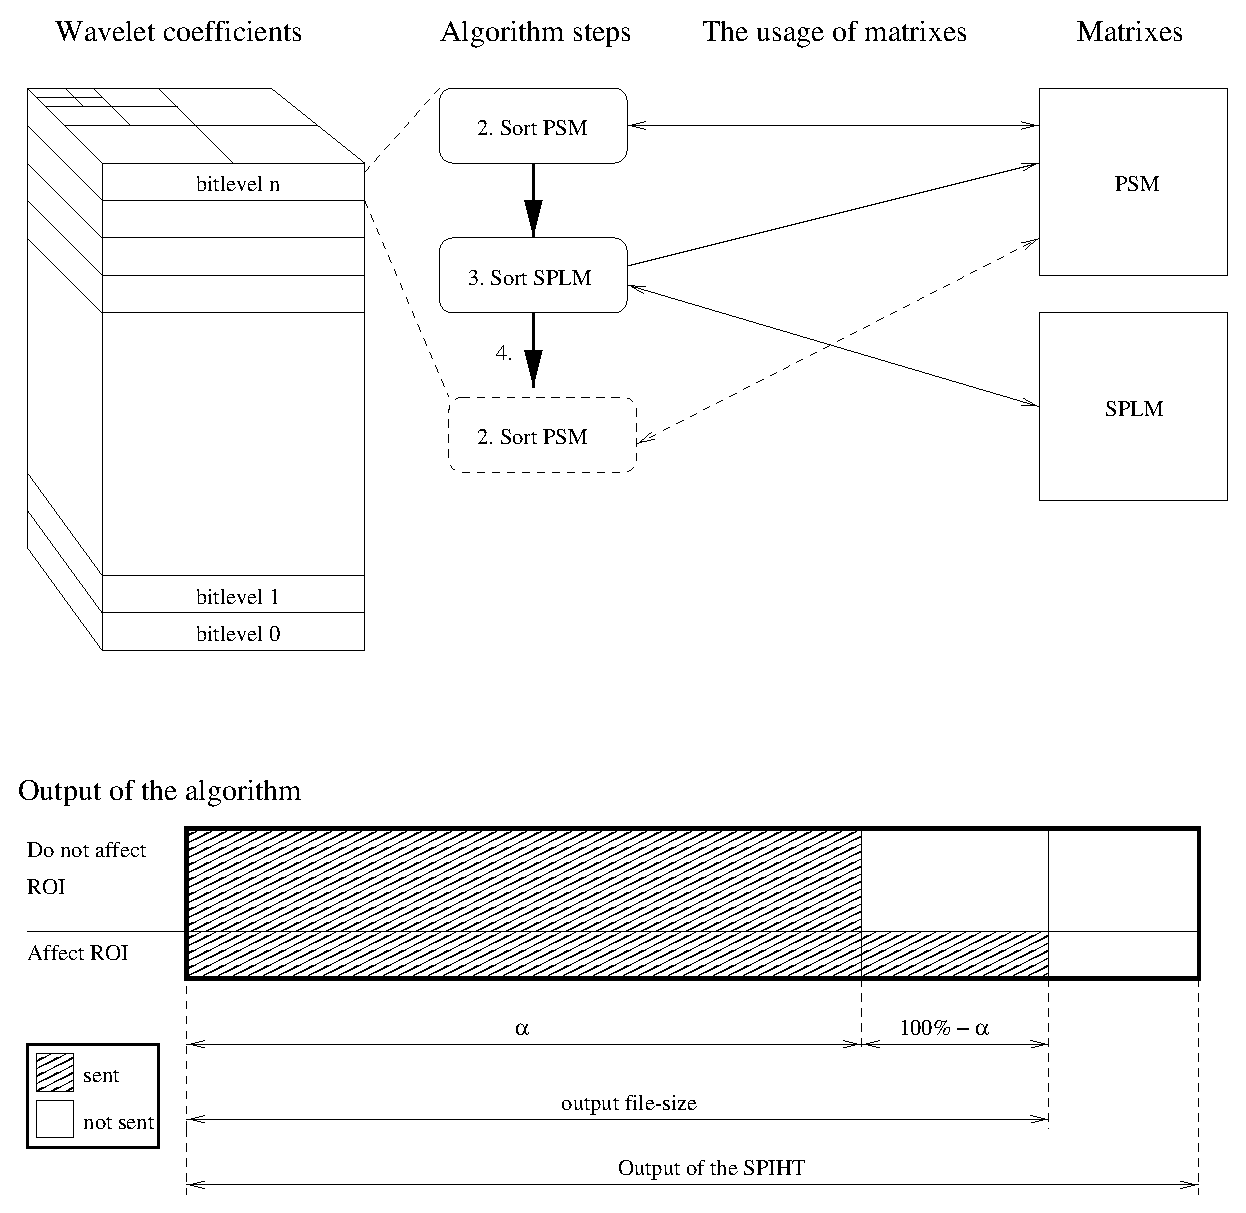
\includegraphics[width=12cm]{algorithm.eps}
\caption{\label{algorithm}}
\end{center}
\end{figure}

\clearpage
\begin{figure}
\begin{center}
\includegraphics[width=12cm]{c_orig.ps}

\caption{\label{orig1}}
\end{center}
\end{figure}

\clearpage


\begin{figure}
\begin{center}
\includegraphics[width=12cm]{c_poster.ps}

\caption{\label{ti1poster}}
\end{center}
\end{figure}

\clearpage

\begin{figure}
\begin{center}
\includegraphics{bigroi.ps}

\caption{\label{bigroi}}
\end{center}
\end{figure}

\clearpage

\begin{figure}
\begin{center}
\includegraphics[width=12cm]{m_whole_original.ps}

\caption{\label{orig2}}
\end{center}
\end{figure}

\clearpage


\begin{figure}
\begin{center}
\includegraphics[width=12cm]{m_segmentation.ps}

\caption{\label{segmentation}}
\end{center}
\end{figure}

\clearpage

\begin{figure}
\begin{center}
\includegraphics[angle=270, width=13cm]{mammo_wholepsnr.ps}

\caption{\label{MSEwhole}}
\end{center}
\end{figure}

\clearpage




\begin{figure}
\begin{center}
\includegraphics[angle=270,width=13cm]{mammo_roipsnr.ps}

\caption{\label{areaMSE}}
\end{center}
\end{figure}
\clearpage

\begin{figure}
\begin{center}
\includegraphics[width=16cm]{small_m_poster.ps}

\caption{\label{ti2poster}}
\end{center}
\end{figure}

\clearpage

\begin{table}
\begin{center}
\begin{tabular}{|l|l|l|l|}
\hline
method 	& bpp 	& PSNR 	& PSNR in ROIs \\
\hline
\hline
GIF 			& 4.456 & $\infty$ 	& $\infty$    \\
JPEG			& 1.01 & 26.01	& 23.76  \\
JPEG			& 0.50 & 23.09	& 20.21  \\
JPEG			& 0.29 & 20.43	& 17.81 \\
SPIHT 			& 1.00 & 27.56 & 26.58 \\
SPIHT 			& 0.50 & 24.06 & 22.13 \\
SPIHT 			& 0.25 & 21.00 & 18.63 \\
vqSPIHT $\alpha = 90 \%$ & 1.00 & 27.26 & 39.85  \\
vqSPIHT $\alpha = 90 \%$ & 0.50 & 23.83 & 29.76 \\
vqSPIHT $\alpha = 90 \%$ & 0.25 & 20.75 & 23.41 \\
vqSPIHT $\alpha = 80 \%$ & 1.00 & 26.72 & 42.46 \\
vqSPIHT $\alpha = 80 \%$ & 0.50 & 23.40 & 34.36 \\
vqSPIHT $\alpha = 80 \%$ & 0.25 & 20.37 & 26.85 \\
vqSPIHT $\alpha = 80 \%$ & 0.15 & 18.55 & 22.13\\
vqSPIHT $\alpha = 80 \%$ & 0.10 & 17.45 & 18.94 \\
vqSPIHT $\alpha = 80 \%$ & 0.05 & 15.15 & 14.55 \\
\hline
\end{tabular}
\end{center}
\caption{Comparison between SPIHT, vqSPIHT and JPEG for the comic
image (Fig.~\ref{orig1}).}
\label{tab1}
\end{table}

\clearpage

{\bf Captions of figures:}

\bigskip

Fig.~\ref{pyramids}. An example of a wavelet coefficient table, that contains
three four-level pyramids: $A$, $B$ and $C$. Scaling coefficients are
located on the square noted by $S$.

\bigskip

Fig.~\ref{algorithm}. The vqSPIHT matrix implementation is illustrated 
on the upper half of the picture: The wavelet coefficients on the left 
are processed one bitlevel at a time. Each bitplane is processed in
two steps (2. and 3.). The first step tests the significance of each coefficient
that is labeled to be insignificant in PSM matrix and transmits the necessary
information. The second step processes all the trees in SPLM and
sets new points in PSM as $significant$ or $insignificant$. 
The bottom part of the picture illustrates the thresholding of
transmitted data. After the alpha limit has been
reached, only bits of coefficients and decision information that
affects the ROI is sent.


\bigskip


Fig.~\ref{orig1}. The original comic test image with three ROIs marked.

\bigskip

Fig.~\ref{ti1poster}. A region of the comic test image containing an ROI
compressed with JPEG, SPIHT and vqSPIHT. See the table below for the
explanation of sub-regions of the figure.

\smallskip
\begin{tabular}{c|c|c}
JPEG 1.00bpp & JPEG 0.50bpp & JPEG 0.25bpp \\
\hline
SPIHT 1.00bpp & SPIHT 0.50bpp & SPIHT 0.25bpp \\
\hline
vqSPIHT $\alpha 90\%$ 1.00bpp & vqSPIHT $\alpha 90\%$ 0.50bpp &
vqSPIHT $\alpha 90\%$ 0.25bpp \\ 
\hline
vqSPIHT $\alpha 80\%$ 1.00bpp & vqSPIHT $\alpha 80\%$ 0.50bpp &
vqSPIHT $\alpha 80\%$ 0.25bpp \\ 
\hline
vqSPIHT $\alpha 80\%$ 0.15bpp & vqSPIHT $\alpha 80\%$ 0.10bpp & ROI in
original \\
\end{tabular}

\bigskip

Fig.~\ref{bigroi}. The two images on the left are ROI masks used in
the compression of the two rightmost images, where ROI covers 16\%
(the upper image) and 46\% of the image. The first grayscale image is
compressed with without ROI ($\alpha = 100\%$), while 16\% ROI ($\alpha
= 50\%$) is used in the second image and 46\% ROI ($\alpha = 50\%$) in
the last image. All the images are compressed with same 0.25 bpp bitrate. 

\bigskip

Fig.~\ref{orig2}. Original mammogram test image.

\bigskip

Fig.~\ref{segmentation}. Micro-calcifications found in the test mammogram (shown as black), and
the ROIs (dotted rectangles around micro-calcifications).

\bigskip


Fig.~\ref{MSEwhole}. PSNR of the whole mammogram for vqSPIHT as a function of
$\alpha$ and bpp.

\bigskip


Fig.~\ref{areaMSE}. PSNR of the ROIs in the  mammogram for vqSPIHT as a function of
$\alpha$ and bpp.

\bigskip

Fig.~\ref{ti2poster}. A region of vqSPIHT compressed mammograms with different
$\alpha$ and bpp rates. Bpp values on
the columns from left to right are 1.00, 0.50 and 0.15. The values of
$\alpha$ starting from the uppermost row are 100\%, 90\%, 70\% and
50\%. All the images have been histogram equalized to ease the
evaluation. The three images in the last row from left to right  are:
the histogram equalized uncompressed region, original uncompressed
region and a bit map of the detected micro-calcifications with the
ROIs marked.

\bigskip

Table~\ref{tab1}. Comparison between SPIHT, vqSPIHT and JPEG for the comic
image (Fig.~\ref{orig1}).

\newpage

{\bf Footnotes}

\bigskip 

1. A common lossless image compression method.

\end{document}




